\documentclass[10pt]{article}
\usepackage[usenames]{color} %used for font color
\usepackage{amssymb} %maths
\usepackage{amsmath} %maths
\usepackage[utf8]{inputenc} %useful to type directly diacritic characters
\usepackage[letterpaper, portrait, margin=1in]{geometry}
\usepackage{graphicx,wrapfig}
\begin{document}
\subsection*{MSDS610 Week 7 Mahout Assignment - Nathan Worsham}
\subsection*{Playing with Mahout's Spark Shell}
I had trouble navigating the Mahout website for at first I could not find the "Quick Start" but in the "Playing with Mahout's Spark Shell" section it gave instructions for installing both Spark and Mahout. The installation in this section for Mahout is different than previous weeks as it says to clone a github repo. Later I did find the quick start and the normal place to download Mahout, but the installation from git isn't that much different. This meant first using \verb|yum install git| to get the package to use git. 
\begin{figure}[!h]
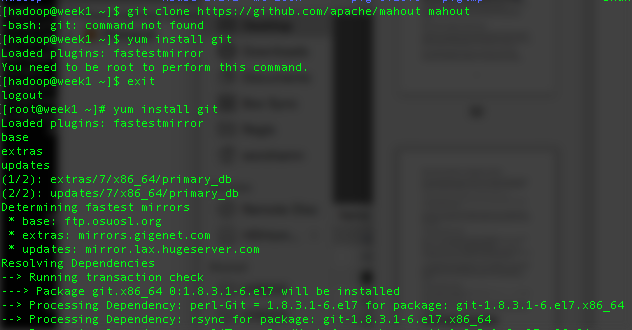
\includegraphics[scale=0.37]{git.png}
\centering
\end{figure}\\
\indent The instructions say to create a directory for Mahout, change to that directory, then clone from git.  But the git command it gives creates a folder anyway, so I elected to just run their command from the home directory of my hadoop user.  
\begin{figure}[!h]
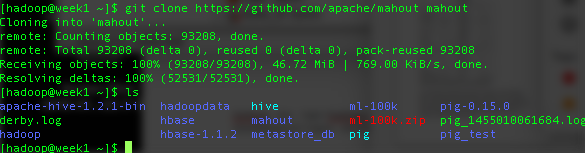
\includegraphics[scale=0.37]{git_mahout.png}
\centering
\end{figure}\\
\indent Now that I had the files from git I was ready to build Mahout with the \verb|mvn| command which to no surprise was not installed. So again I switched to root and installed it--I ended up needing to use \verb|yum provides mvn| to find that it was part of the "maven" package. 
\begin{figure}[!h]
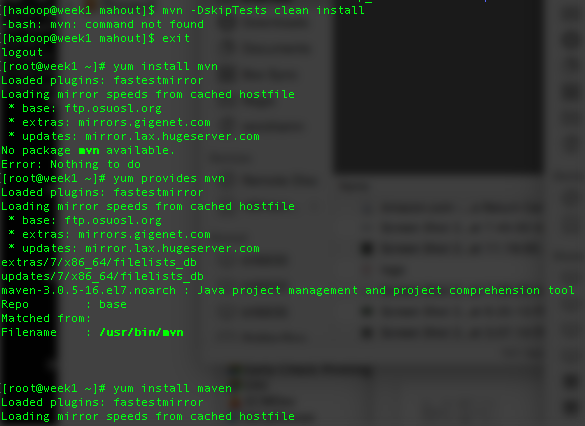
\includegraphics[scale=0.37]{install_maven.png}
\centering
\end{figure}\\
\indent Trying to build using the maven package, I received a build error. After looking at a stackoverflow.com thread (2015), I realized that the maven I installed was an older version and that Mahout has a requirement for a newer version. I went ahead and tried to update through yum but there were no updates for maven through the regular yum repos. 
\par
\raisebox{-.6\height}{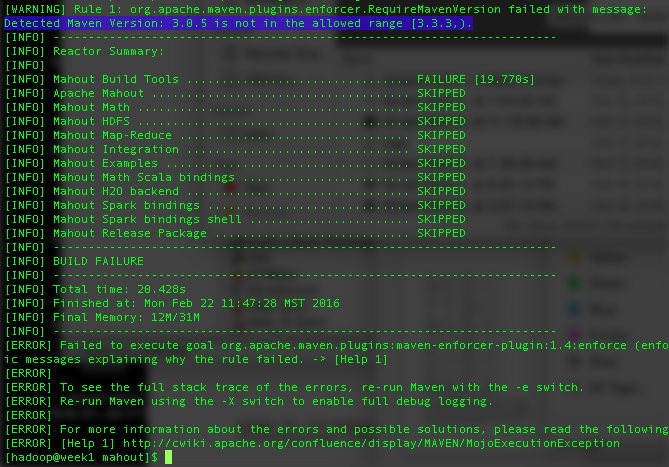
\includegraphics[width=8cm]{build_failure.png}}%
\hfill
\raisebox{-.6\height}{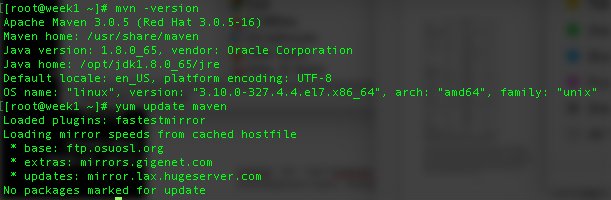
\includegraphics[width=8cm]{no_update_maven.png}}%
\par
So following another site (gluster.org, 2013) instructions for installing the latest maven through yum, I downloaded a new repo and then used \verb|yum install apache-maven|. But again I received some errors, this time because it was conflicting with some the dependencies that were installed for the previous maven. I went ahead and ran \verb|yum autoremove| to get rid of the old dependencies and then I was able to install apache-maven. The article then said to update symlinks for mvn but did not say how or where to do it. I went ahead and just created a single symbolic link to \verb|/usr/local/bin/mvn| since I knew that was in the PATH. Now I was able to run the mvn command, a command that took a long time to complete, downloaded quite a bit of content and expressed several warning messages, but ultimately did say the build was a success.
\par
\raisebox{-.6\height}{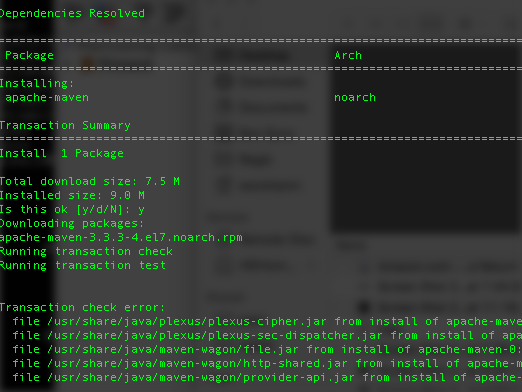
\includegraphics[width=8cm]{yum_errors.png}}%
\hfill
\raisebox{-.6\height}{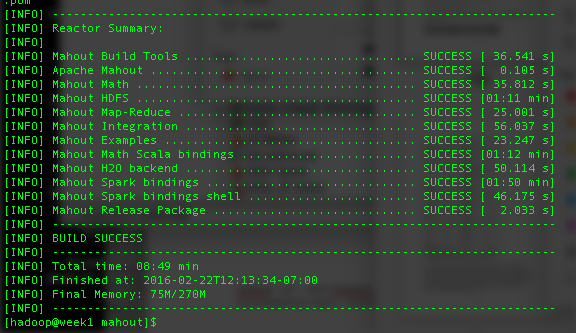
\includegraphics[width=8cm]{build_success.png}}%
\par
Next it had me start Spark and confirm by going to a local webpage--which is something I did not see last week. After trying for a bit to get to port 8080, I realized the local firewall was in the way and I elected to simply turn it off with \verb|service firewalld stop|. After that I was to copy the URL in order to place it into an environment variable which I did.
\par
\raisebox{-.6\height}{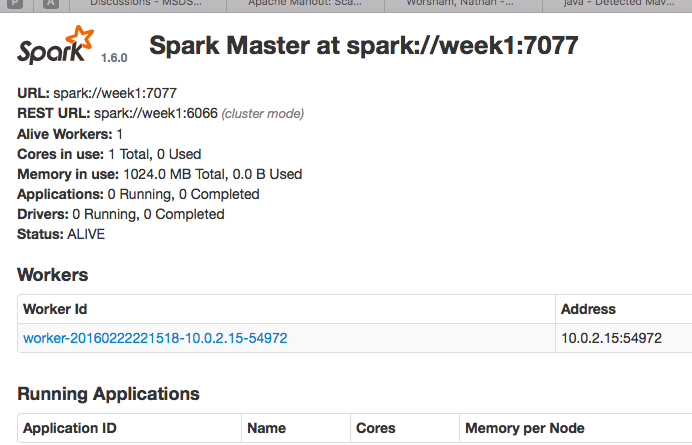
\includegraphics[width=8cm]{spark_site.png}}%
\hfill
\raisebox{-.6\height}{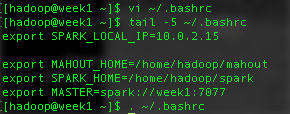
\includegraphics[width=8cm]{environment.png}}%
\par
Now I was ready to try to get to the \verb|mahout spark-shell|. The first time I tried it I received an error about trying to connect to localhost on port 9000, which made me realize I had better start up HDFS and yarn (as the instructions did not indicate but was maybe implied). After starting those services and trying again I received a much better result because I got back the \verb|mahout>| prompt. However I did receive a couple of warnings about plugins already being registered and failing to get a database default.
\begin{figure}[!h]
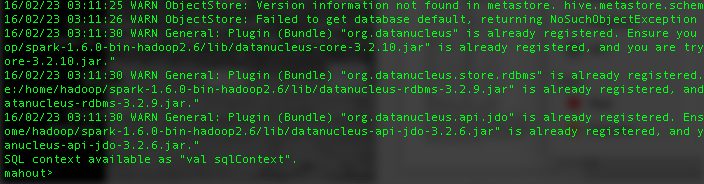
\includegraphics[scale=0.37]{already_registered.png}
\centering
\end{figure}\\
\indent The next step in the exercise was to setup a matrix that represented ingredients (protein, fat, carbohydrate and sugars in milligrams) of various cereals, along with a column of combined user ratings of the cereals. The purpose of the exercise is to fit a linear model which infers the customer rating from the ingredients using a linear regression algorithm. I created the matrix and pulled out the X and Y values into variables.
\begin{figure}[!h]
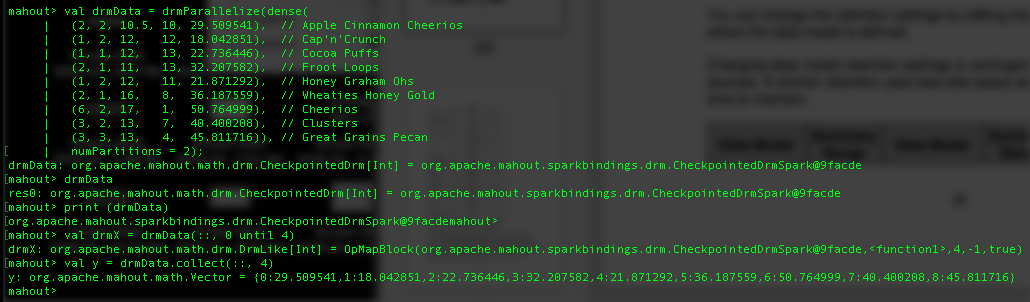
\includegraphics[scale=0.37]{setup.png}
\centering
\end{figure}\\
\indent Using Ordinary Least Squares, I then created variables containing matrix multiplication so that the two variables could then be multiplied to find "beta". What is interesting is after making the variable the equation for each value, I then have to run a "collect" command in order to fetch the values into memory so that the solve function can be run on them.
\begin{figure}[!h]
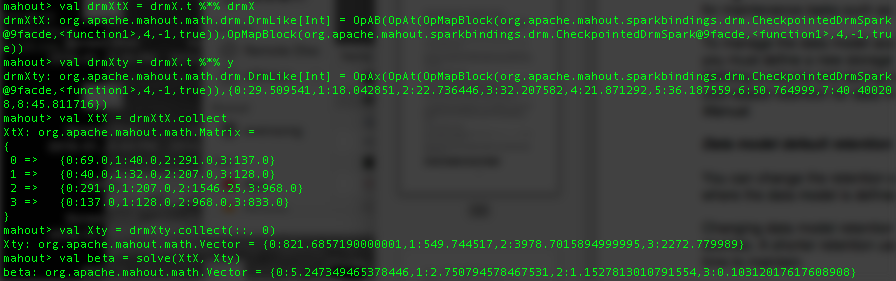
\includegraphics[scale=0.37]{equation.png}
\centering
\end{figure}\\
\indent Now I was to check how well the model fits by first multiplying the ingredient features by the estimated beta (yFitted), and then by looking at the difference between actual y and fitted y using something called L2-norm. I receive an answer of about 14.2. Looking for information on L2-norm brought me to a blog post (Rorasa, 2015) that essentially stated that it is also known as Euclidean distance.
\begin{figure}[!h]
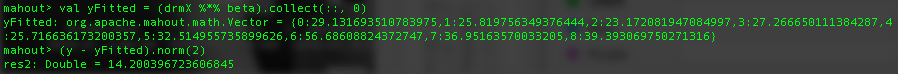
\includegraphics[scale=0.37]{fit1.png}
\centering
\end{figure}\\
\indent The next part in the exercise was to refactor everything that was just done into two functions and then also add a constant bias term to the model. The result was a goodness of fit of nearly half of what it previously was at approximately 7.6.
\pagebreak
\begin{figure}[!h]
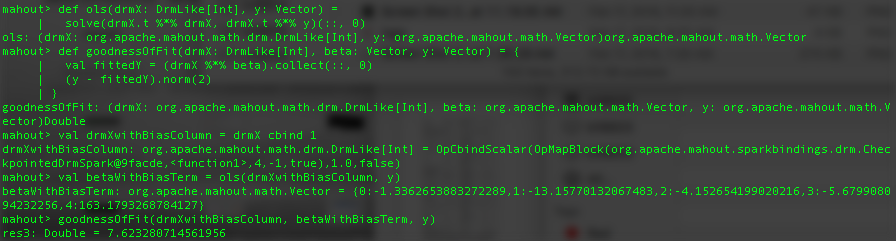
\includegraphics[scale=0.37]{fit2.png}
\centering
\end{figure}\\
\indent Last the exercise was to implement a caching functionality to cache the value of the bias column into memory. This was for improved performance as it resulted in the same outcome.
\begin{figure}[!h]
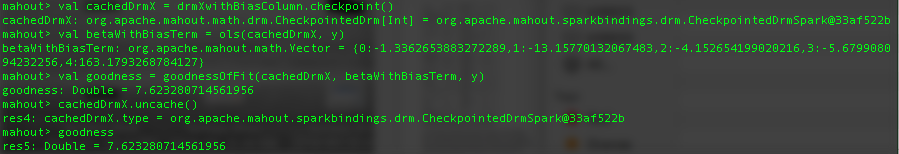
\includegraphics[scale=0.37]{fit3.png}
\centering
\end{figure}\\
\subsection*{Twenty Newsgroups Classification Example}
After completing the Spark shell exercise, I was really just interested in poking around the other exercises to see if anything looked interesting. I ended up trying the newsgroups classification exercise, which takes a dataset collection of about 20,000 newsgroup documents and classifies them into 20 different newsgroups. The exercise starts off with just having you run one of the examples contained within the Mahout folder. I went ahead and tried running the \verb|./examples/bin/classify-20newsgroups.sh| script but I ended up receiving an error about the "temp/weights" folder not being publicly accessible. I took that to mean that it was not a world writable folder, so I tried \verb|chmod 777| the rights of the folder and ran the example again but I received the same error. 
\begin{figure}[!h]
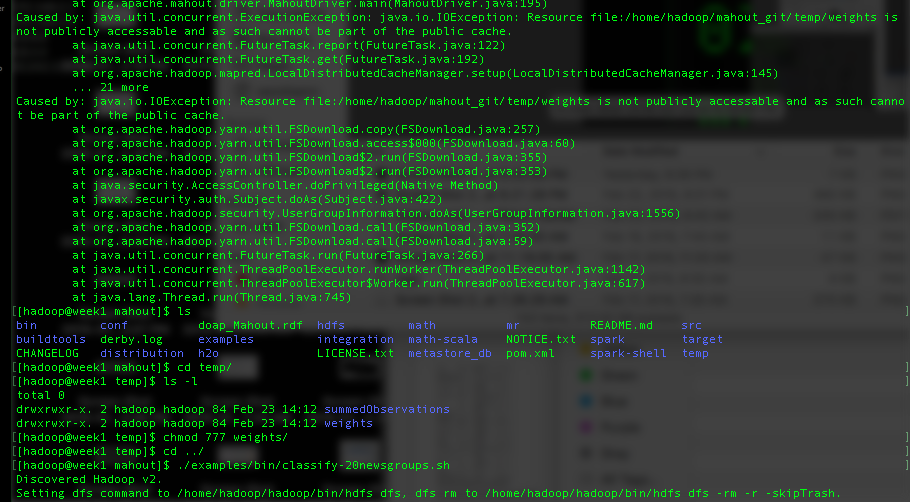
\includegraphics[scale=0.37]{classify1.png}
\centering
\end{figure}\\
\indent Even after opening the rights on the folder, when I ran the example again the folder's rights went back to the way they were (775), so the script must have a bug I'm guessing. At this point I decided to walk through the example as they gave step-by-step instructions for how the example script works. I first checked to see if I could find the file the script already downloaded but could not find it as it took awhile to download. I then set the environment variables accordingly and made the working directory.
\pagebreak
\begin{figure}[!h]
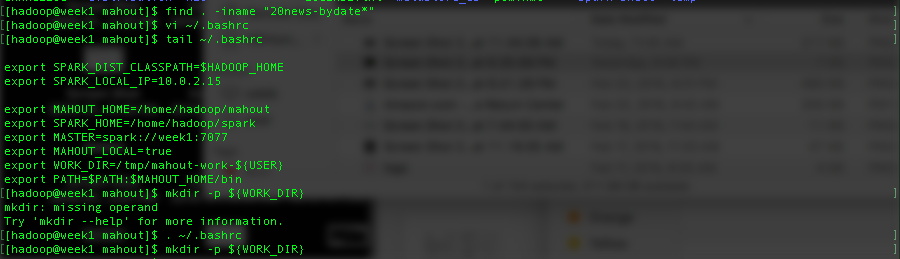
\includegraphics[scale=0.37]{classify2.png}
\centering
\end{figure}\\
\indent Next I re-downloaded the data set, unpacked it, and then tried to make another required directory that apparently already existed. 
\begin{figure}[!h]
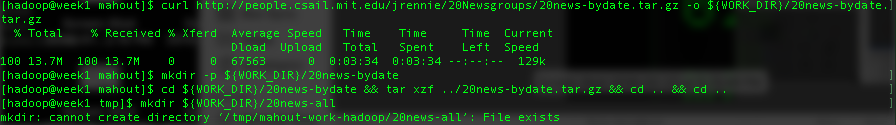
\includegraphics[scale=0.37]{classify3.png}
\centering
\end{figure}\\
\indent The instructions had an optional section about trying to "put" a folder and contents into the HDFS, but it seems the command is deprecated and it complained of "No such file or directory". Given that it was optional, I decided to move on without it.
\begin{figure}[!h]
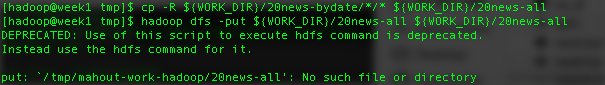
\includegraphics[scale=0.37]{hadoop_put.png}
\centering
\end{figure}\\
\indent I then successfully ran the commands to convert the dataset into a sequence file and then a sequence file with term frequencies for each document.
\par
\raisebox{-.6\height}{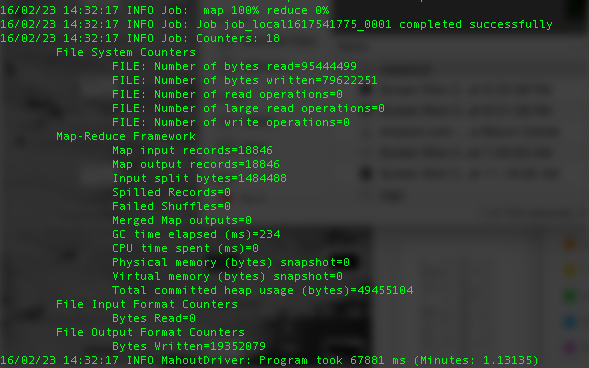
\includegraphics[width=8cm]{seqdirectory.png}}%
\hfill
\raisebox{-.6\height}{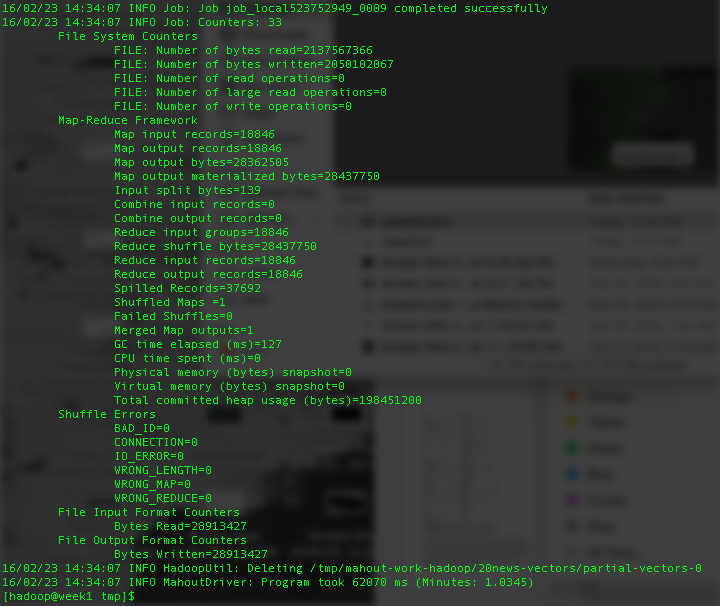
\includegraphics[width=8cm]{seq2sparse.png}}%
\par
Split the dataset into training and testing sets.
\pagebreak
\begin{figure}[!h]
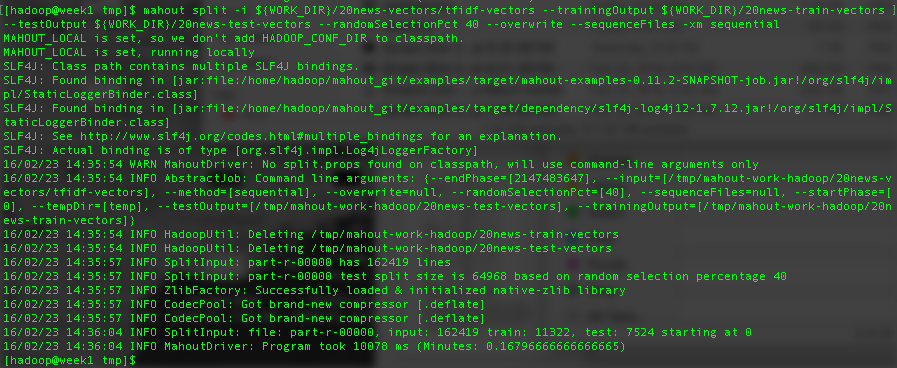
\includegraphics[scale=0.37]{split.png}
\centering
\end{figure}\\
\indent When I tried to run the command to train the classifier I received an error complaining about the \verb|-el| option, so not really knowing what to do, I decided to simply remove the option which luckily still worked. 
\par
\raisebox{-.6\height}{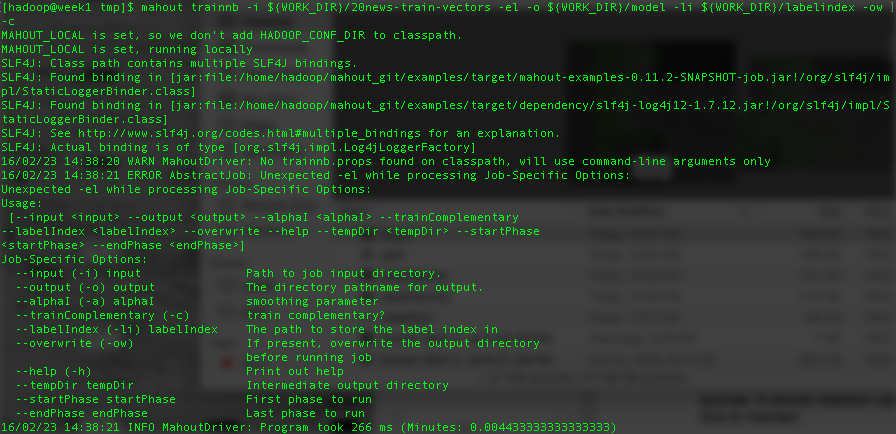
\includegraphics[width=8cm]{with_el.png}}%
\hfill
\raisebox{-.6\height}{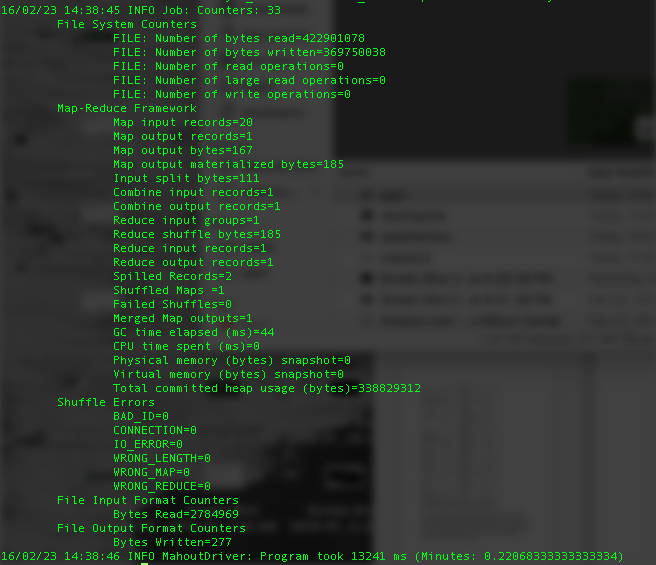
\includegraphics[width=8cm]{no_el.png}}%
\par
Finally I was able to test the classifier and received the output that the example script did not supply.
\begin{figure}[!h]
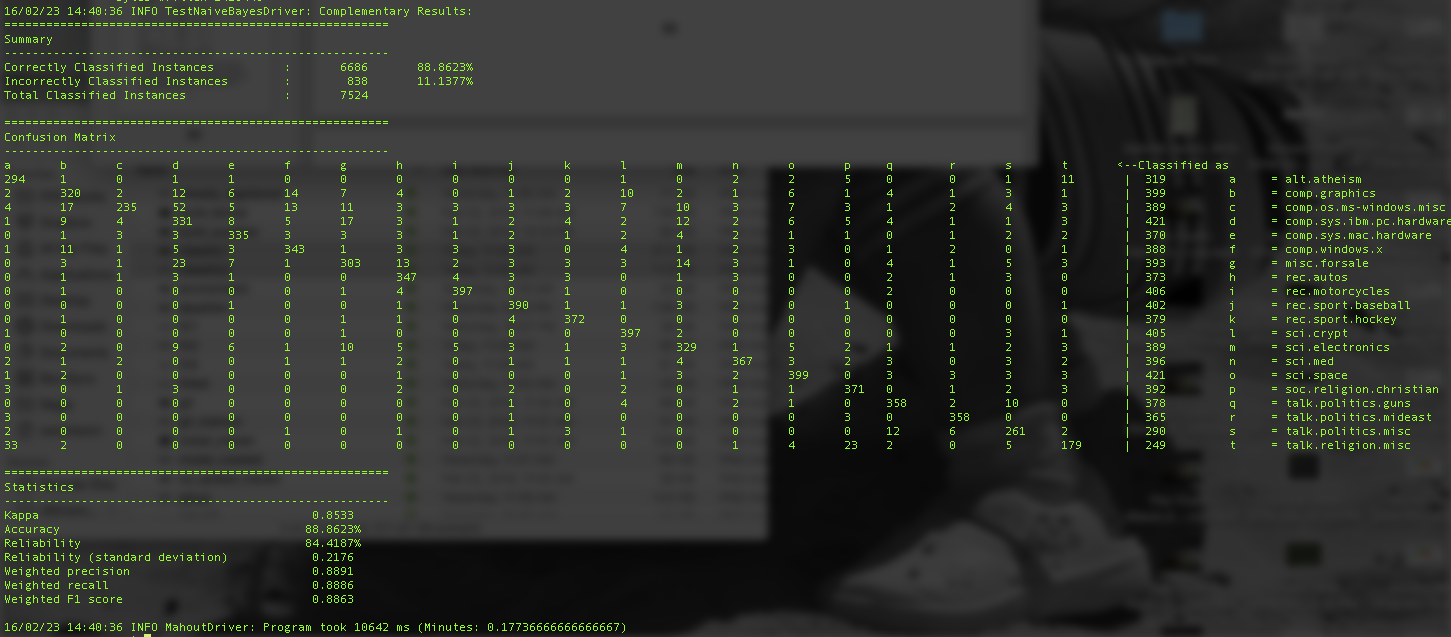
\includegraphics[scale=0.37]{complete.png}
\centering
\end{figure}\\
\subsection*{References}
stackoverflow.com, 2015. Retrieved from http://stackoverflow.com/questions/31968515/detected-maven-version-3-0-5-is-not-in-the-allowed-range-3-2\\
rorasa.wordpress.com, 2015. Retrieved from https://rorasa.wordpress.com/2012/05/13/l0-norm-l1-norm-l2-norm-l-infinity-norm/\\
mahout.apache.org, 2016. Retrieved from http://mahout.apache.org/users/sparkbindings/play-with-shell.html\\
and http://mahout.apache.org/users/classification/twenty-newsgroups.html
\end{document}
